\chapter{矩阵乘GPU实现}\label{chap:GEMMGPU}

%我们使用外积(outer product)法计算矩阵乘。因为外积法比內积法(inner product)在GPU上的并行性好。例如,我们要计算下面的矩阵乘法C=AxB。使用內积法,我们需要按照下面的公式计算:
本文使用外积(outer product)法计算矩阵乘。因为外积法比內积法(inner product)在GPU上的并行性好。例如,要计算下面的矩阵乘矩阵$C=A \times B$。使用內积法,需要按照下面的公式计算:

\begin{equation}
\label{eq:innerproduct}
C[i][j]=\sum_{k}A[i][k]B[k][j]
\end{equation}

%我们可以并行的计算所有的乘法,但不能并行的计算加法。即使我们可以使用reduction来快速计算加法,但仍然会产生很多空闲的线程。这样,由于任务划分的不均衡,会使得计算性能大大降低。然而,如果我们用外积法来代替內积法,将会很大程度上缓解负载不均衡带来的性能损失。下面是外积法的计算公式:
采用內积法可以并行的计算所有的乘法,但不能并行地计算加法。即使可以使用reduction来快速计算加法,但仍然会产生很多空闲的线程。这样,由于任务划分的不均衡,会使得计算性能大大降低。然而,如果用外积法来代替內积法,将会很大程度上缓解负载不均衡带来的性能损失。下面是外积法的计算公式:

\begin{equation}
\label{eq:outerproduct}
C^{(k)}=A[:][k]B[k][:], C=\sum_{k}C^{(k)}
\end{equation}

在计算A[:][k]B[k][:]时,每个线程只需负责读取A的一个小块和B的一个小块,来计算对应C的一个小块;每个线程可以独立的将当前计算得到的C的一小块的部分和累加到对应C的一小块上。当C的部分和全部都累加起来时,我们一次性写回C到全局内存。

%在算法设计上,我们采用外积法, A矩阵列优先存储,B矩阵行优先存储, 图\ref{fig:outer_product}为一个block中的线程读取A,B中的数据块, 和对应到C矩阵的输出
在算法设计上,本文采用外积法, A矩阵列优先存储,B矩阵行优先存储, 图\ref{fig:outer_product_replot}为一个block中的线程读取A,B中的数据块, 和对应到C矩阵的输出。

%问题定义: C = A * B, A大小为MxK, B为KxN, C为MxN 
问题定义: $C = A * B$, A大小为$M \times K$, B为$K \times N$, C为$M \times N$

矩阵乘外积法:用A矩阵的一列乘以B矩阵的一行,沿着K方向做累加,可以计算出结果C(图\ref{fig:outer_product_replot})。
\begin{figure}[htbp]
	\centering
	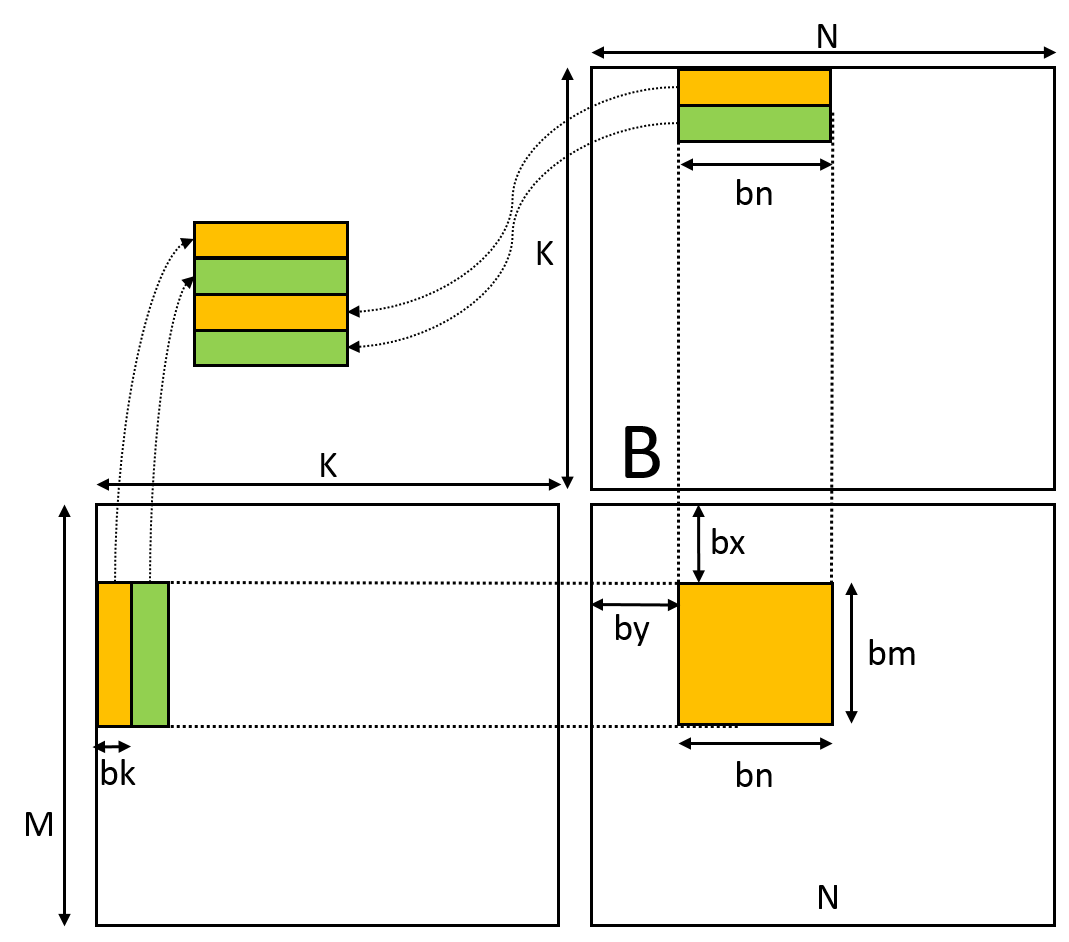
\includegraphics[width=0.50\textwidth]{outer_product_replot}
	\bicaption{矩阵乘外积法图示}{Illustration of Outer-product matrix multiplication method}
	\label{fig:outer_product_replot}
\end{figure}
\section{矩阵乘外积法算法描述}

%\begin{algorithm}[htbp]
%	\small
%	\caption{GEMM algorithm}\label{alg:gemm}
%	\begin{algorithmic}[1]
%		%\Procedure{Euclid}{$a,b$}\Comment{The g.c.d. of a and b}
%		\State preload block of A, B
%		\While{one more valid block of A, B exists}
%		\State load block of A, B from global memory to registers
%		\State store block of A, B from registers to shared memory
%		\State load block of A, B from shared memory to registers
%		\State compute block of C in registers
%		\EndWhile\label{gemmendwhile}
%		\State store C from registers to global memory
%		%\EndProcedure
%	\end{algorithmic}
%\end{algorithm}

\begin{algorithm}[htbp]
	\small
	\caption{GEMM algorithm}\label{alg:gemm}
	\begin{algorithmic}[1]
		%\Procedure{Euclid}{$a,b$}\Comment{The g.c.d. of a and b}
		\State $A, B, C$\Comment{matrix A, B, C}
		\State $regA[task\_size],regB[task\_size],regC[task\_size]$\Comment{Allocate register for compute}
		\State $tileA[tile\_size],tileB[tile\_size]$\Comment{Allocate shared memory for tile of A, B}
		\State $regC \gets 0$
		\While{one more valid block of A, B exists}
%		\State load block of A, B from global memory to registers
%		\State store block of A, B from registers to shared memory
%		\State load block of A, B from shared memory to registers
%		\State compute block of C in registers
        \State $tileA \gets A, tileB \gets B $\Comment{Load tile of A, B from global to shared}
        \State barrier
        \For   {$k = 0$; $k<NUM\_UNROLL$;$++k$}\Comment{Loop Unroll}
        \State $regA \gets tileA, regB \gets tileB$
        \State $regC \gets regA \cdot regB + regC$
        \EndFor
        \State barrier
		\EndWhile\label{gemmendwhile}
		\State $C \gets regC$\Comment{Store C from registers to global memory}
		%\EndProcedure
	\end{algorithmic}
\end{algorithm}

在算法\ref{alg:gemm}执行上,我们经过下面的步骤:

(1)	数据预取,从全局内存读取A,B矩阵数据块到寄存器。

(2) 循环开始:

\qquad(2.1) 从全局内存读取A,B数据块到寄存器。

\qquad(2.2) 将读取到寄存器的数据写回的共享内存。

\qquad(2.3) 从共享内存读取A,B数据块到寄存器。

\qquad(2.4) 在寄存器中计算结果C。

\qquad 直到所有的A,B数据块都读取完。

(3) 最后把C的结果从寄存器写回到全局内存。


\section{从全局内存读取数据到共享内存}
全局内存是对所有线程可见,共享内存是对一个线程块里的线程是可见的,寄存器是对线程私有的。从全局内存读取数据到寄存器,然后到共享内存,是为了通过数据分享共享内存的数据,减少慢速的全局内存的访问次数,改为共享内存的访问。展示了线程块从矩阵A和B读取数据到共享内存的过程。线程块分别从矩阵A和矩阵B读取bmxbk和bkxbn的数据,然后使用外积法计算。为了隐藏全局访存的延迟,我们采用软流水和共享内存双缓冲机制。共享分块的大小与GPU上的计算资源如寄存器大小和共享内存大小有关。由于指令不能直接从全局访存读取到共享内存,需要寄存器中转,因此需要分两个步骤。

\subsection{线程到数据的映射}

\begin{figure}[htbp]
	\centering
	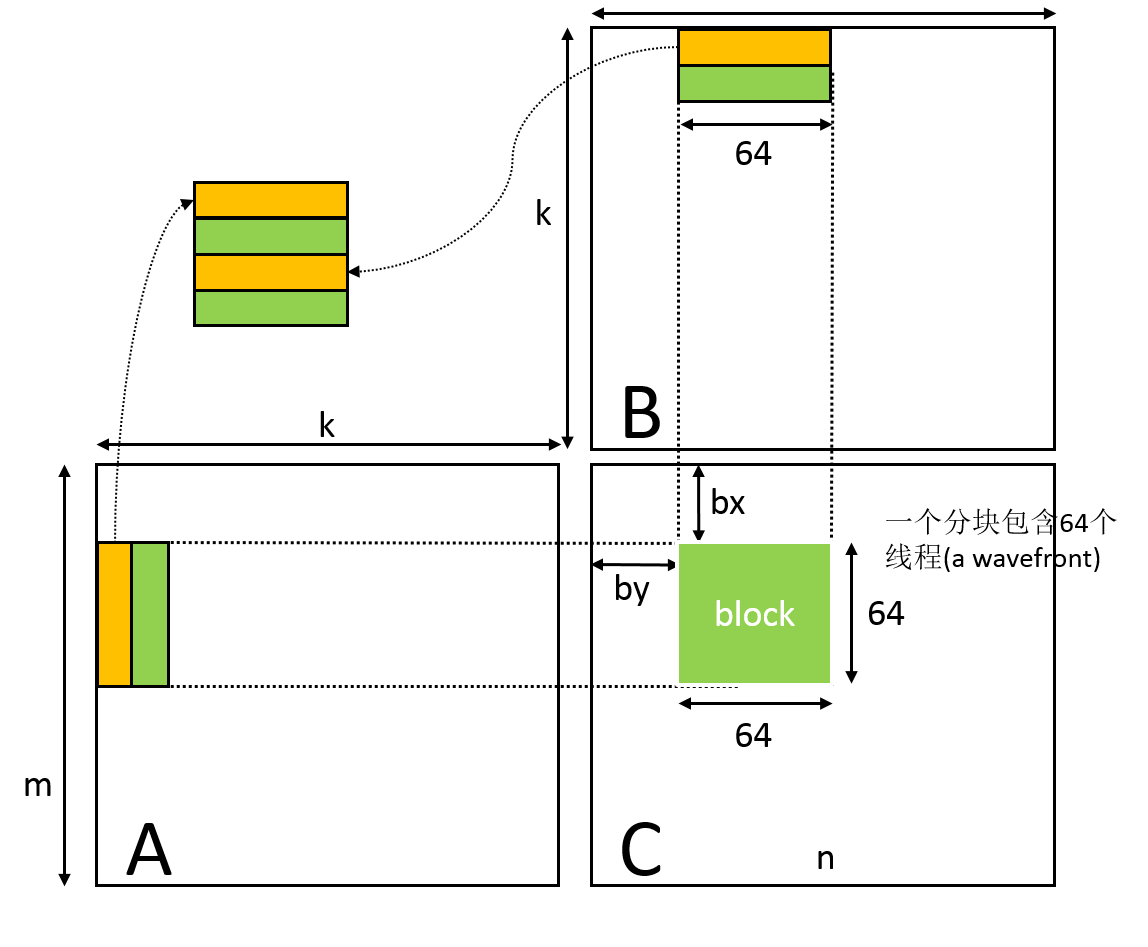
\includegraphics[width=0.50\textwidth]{thread_to_data_replot}
	\bicaption{线程到数据映射}{Thread-to-data mapping}
	\label{fig:thread_to_data_replot}
\end{figure}

64个线程(即一个wavefront)组成一个block,每个线程计算8x8的输出,一个block共计算64x8x8=64x64的输出(如图\ref{fig:thread_to_data_replot})。

\begin{figure}[htbp]
	\centering
	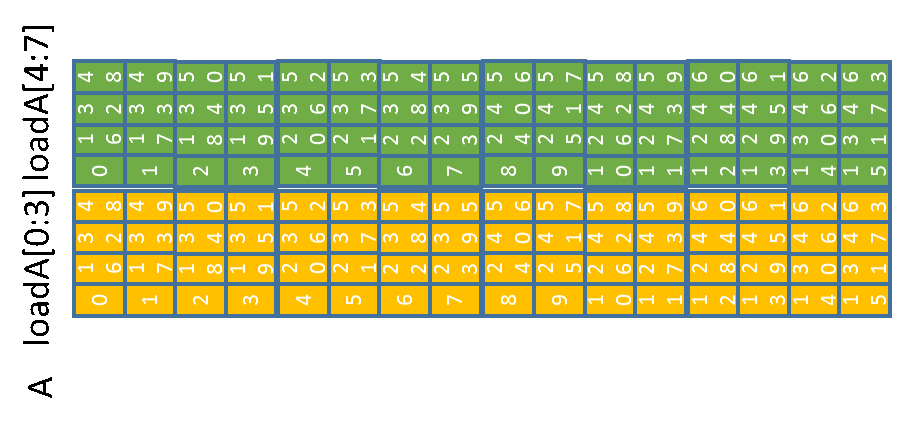
\includegraphics[width=0.50\textwidth]{global_A}
	\bicaption{从全局内存读取A矩阵数据到寄存器}{Read A-matrix data from global memory to registers}
	\label{fig:global_A}
\end{figure}

\begin{figure}[htbp]
	\centering
	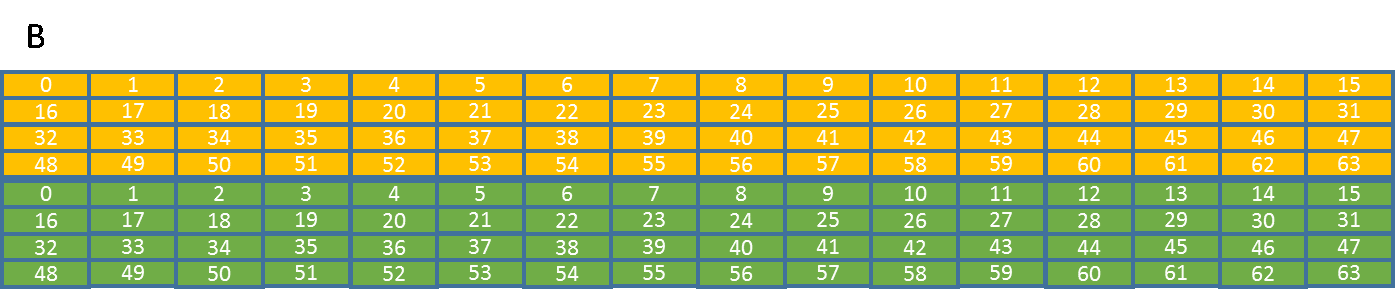
\includegraphics[width=0.50\textwidth]{global_B}
	\bicaption{从全局内存读取B矩阵数据到寄存器}{Read B-matrix data from global memory to registers}
	\label{fig:global_B}
\end{figure}

A(表示保存A矩阵数据的寄存器) : 从全局内存读A数据到寄存器(如图\ref{fig:global_A})

B(表示保存B矩阵数据的寄存器) : 从全局内存读B数据到寄存器(如图\ref{fig:global_B})

图中,小方格中的数字表示threadblock中的线程号。黄色表示已经把全局内存中的数据加载到了寄存器,绿色表示下一次计算需要用到的数据(还没加载好)。黄色和绿色构成寄存器双缓冲。

\begin{figure}[htbp]
	\centering
	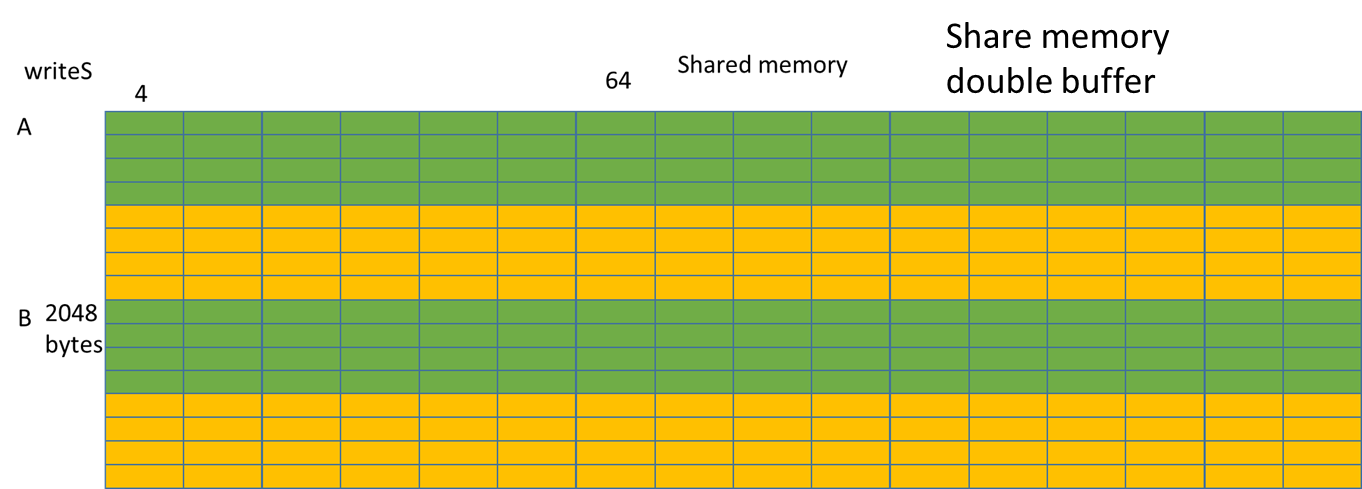
\includegraphics[width=0.50\textwidth]{writeS}
	\bicaption{写回A,B数据到共享内存}{Write A,B to shared memory}
	\label{fig:writeS}
\end{figure}

将寄存器中读好的A,B写回到局部共享内存。图\ref{fig:writeS}中绿色表示正在从寄存器写回数据到局部共享内存,黄色表示下一次要写回到局部共享内存的地址。黄色和绿色构成局部共享内存双缓冲。


\section{从共享内存读取数据到寄存器并计算}
矩阵A,B是否转置只与读取全局内存有关,一旦数据存储到共享内存,访问无关。所以从此步骤之后,论述任务划分时,不再区分矩阵A,B是否转置。
\begin{figure}[htbp]
	\centering
	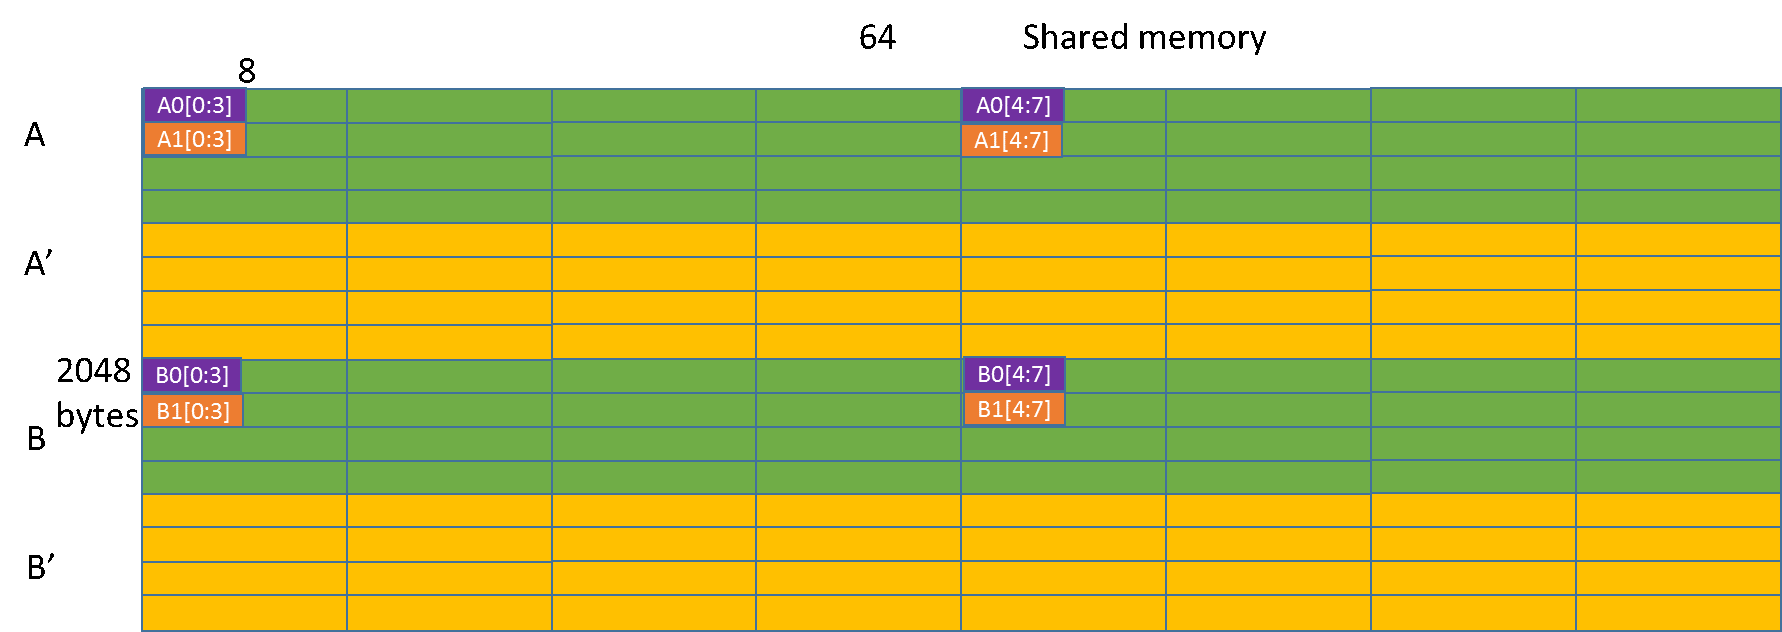
\includegraphics[width=0.50\textwidth]{readS}
	\bicaption{从共享内存读取A,B数据到寄存器}{Read A,B from shared memory to registers}
	\label{fig:readS}
\end{figure}

接下来就可以计算矩阵C了。图\ref{fig:readS}中紫色和橙色表示0号线程从局部共享内存要读取的数据。由于前面讲到了循环展开8次,紫色表示偶数次要读取的数据,橙色表示奇数次读取的数据绿色表示数据已经在共享内存中了,可以直接读取,黄色表示双缓冲的另外一半。

\begin{figure}[htbp]
	\centering
	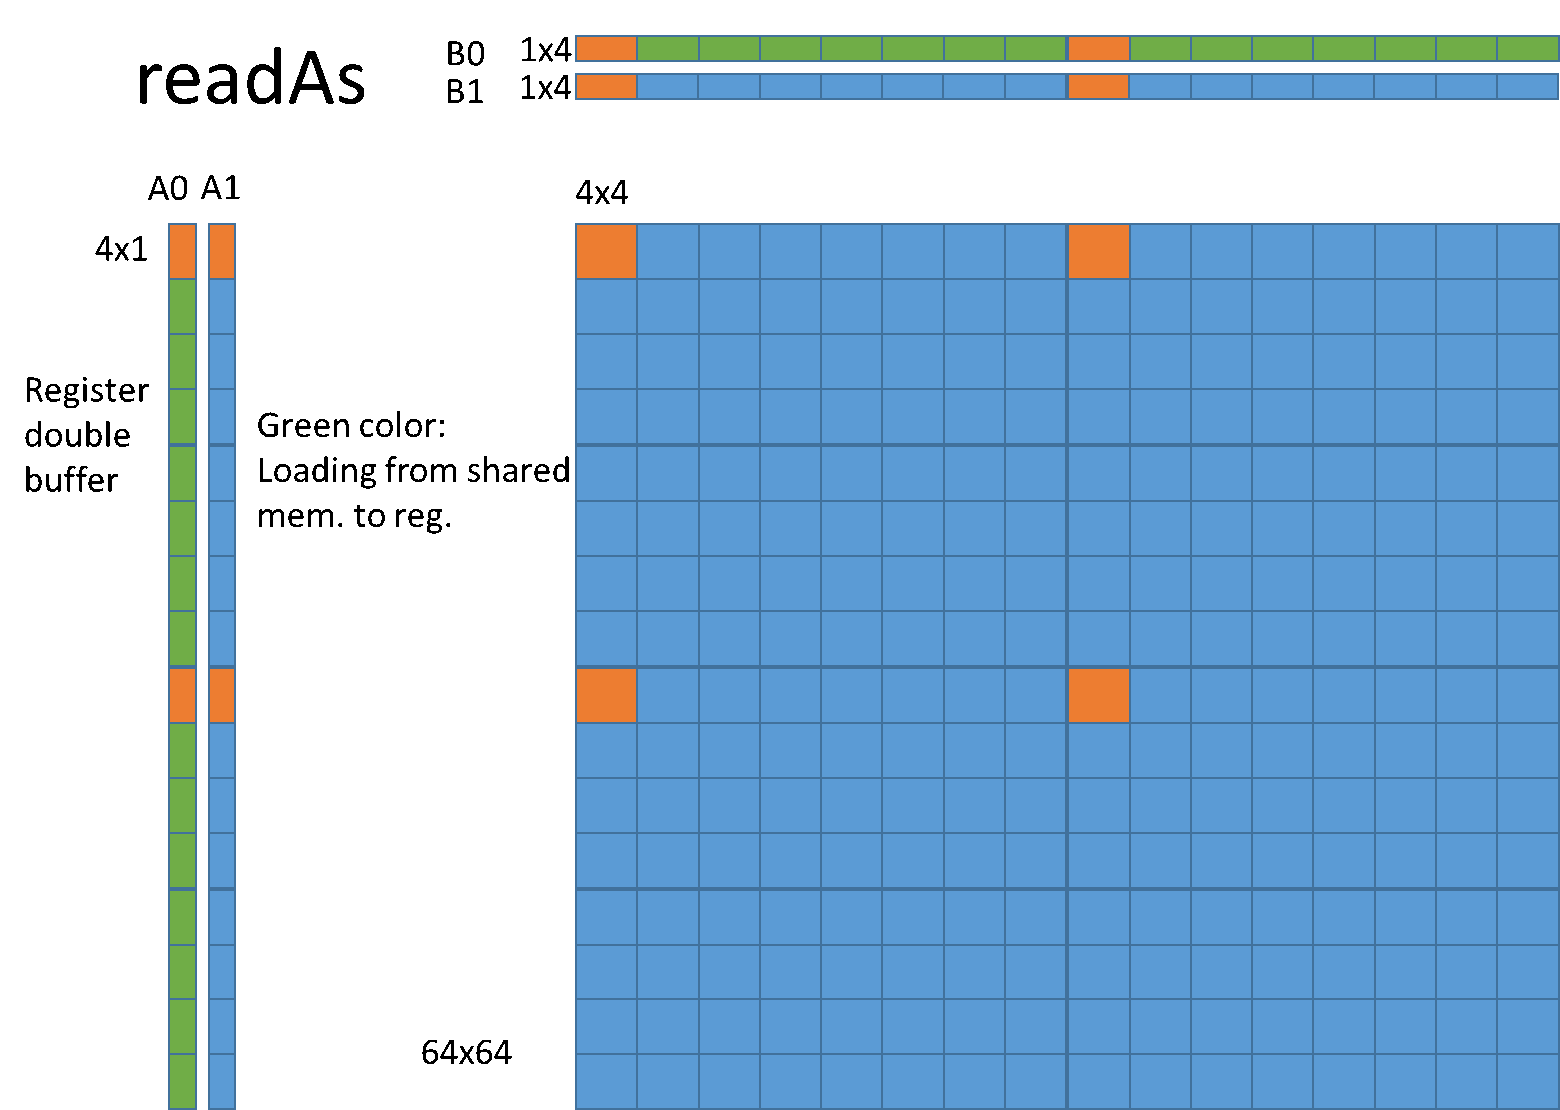
\includegraphics[width=0.50\textwidth]{threadblock}
	\bicaption{一个threadblock中的计算任务}{Computation tasks in a threadblock}
	\label{fig:threadblock}
\end{figure}

从block的角度观察每个线程的计算任务(如图\ref{fig:threadblock})。现在从一个block的角度来观察每个线程计算C的方式,这里一个block由一个wavefront组成,即64个线程, 一个block总共计算64x64个C中元素。图中橙色部分表示0号线程的计算任务,0号线程计算8x8的C,为了线程的负载均衡,这里将8x8分成4个4x4。这里总结一下:我们用了到数据预取、寄存器双缓冲、局部共享内存双缓冲、bank冲突消除、线程负载均衡这些优化方法。


\section{将C矩阵从寄存器写回数据到全局内存}
当循环k/64次,每个线程块就可以把每个小块计算完成。此时需要把C存回全局内存。由于寄存器是私有的,每个线程只能存储自己计算的结果到对应的内存。可以做的优化是把C先从寄存器存回到共享内存,此时线程可以访问同一个线程块内的其他线程的计算结果。然后再从共享内存存储到全局访存。由于此时共享内存中的矩阵A和B的值以后将不再使用,所以不用开辟新的空间,直接复用A,B的空间即可。
通过乘加运算得到最终的结果C矩阵后,一般有两种方式将结果写回全局内存。第一种是先将C矩阵从寄存器写回到共性内存,然后再写回到全局内存;第二种是直接将C矩阵从寄存器写回到全局内存。
首先做4个v\_mul操作,将结果乘以系数alpha。然后用指令tbuffer\_store\_format\_xyzw依次写回4个结果。一个block总共需要写回64个元素,每4条v\_mul指令之间插入一条tbuffer\_store\_format\_xyzw指令。所有block并发执行,将整个C矩阵写回到全局内存。


\section{本章小结}
本章主要讲述了矩阵乘GPU实现的算法和具体实现步骤。描述了矩阵乘外积法的执行过程,并对比分析了外积法相比于內积法的优势。通过三个步骤讲述了外积法矩阵乘算法的数据的搬运和计算的执行过程。线程的映射关系,需要考虑全局访存能否联合访存,共享内存是否有bank冲突,如果遇到非分块整数倍的情况,任务能否均衡。根据本章提供的信息,读者可以复现本文的工作。